% Title: gl2ps_renderer figure
% Creator: GL2PS 1.4.0, (C) 1999-2017 C. Geuzaine
% For: Octave
% CreationDate: Thu May 27 01:15:46 2021
\setlength{\unitlength}{1pt}
\begin{picture}(0,0)
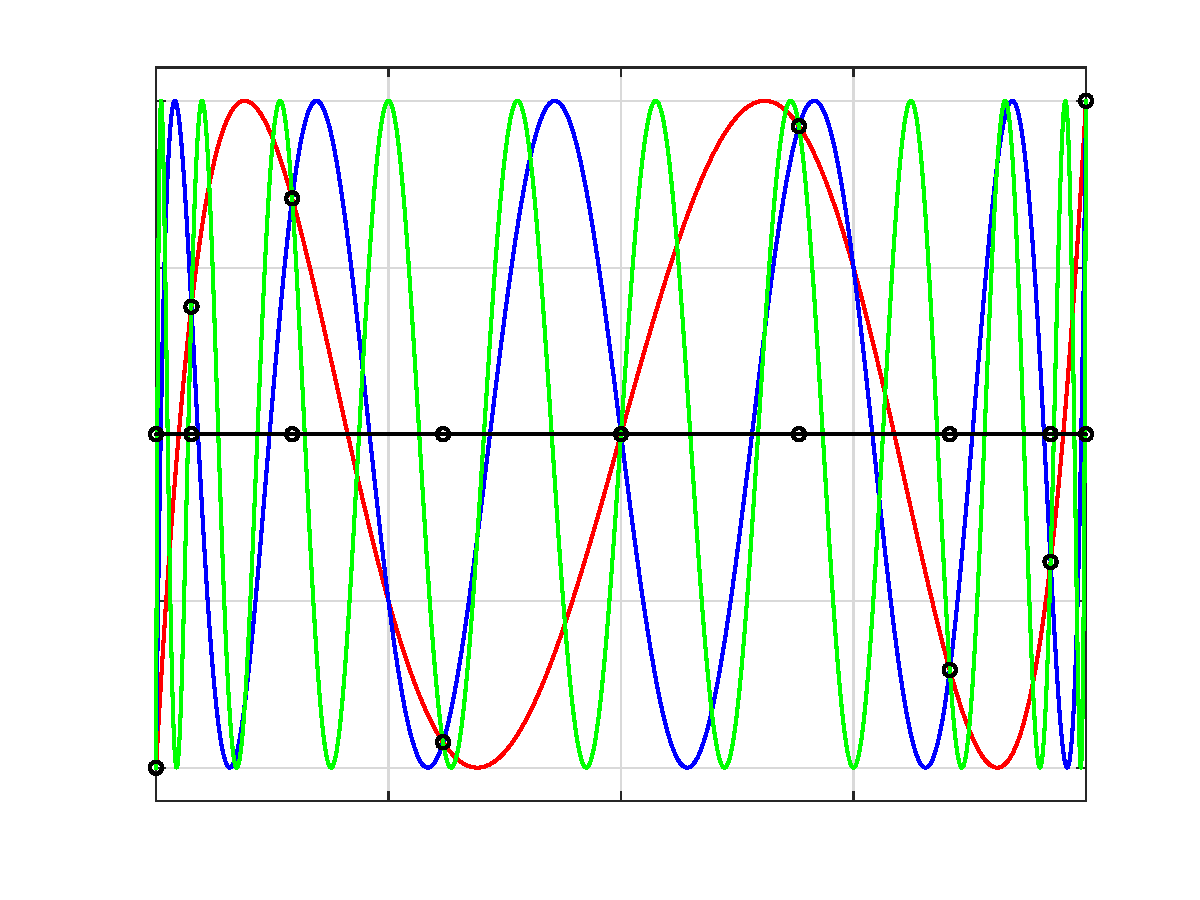
\includegraphics{figures/chap26/OUT/ChebyshevAlias8-inc}
\end{picture}%
\begin{picture}(576,432)(0,0)
\fontsize{10}{0}
\selectfont\put(74.88,40.0183){\makebox(0,0)[t]{\textcolor[rgb]{0.15,0.15,0.15}{{-1}}}}
\fontsize{10}{0}
\selectfont\put(186.48,40.0183){\makebox(0,0)[t]{\textcolor[rgb]{0.15,0.15,0.15}{{-0.5}}}}
\fontsize{10}{0}
\selectfont\put(298.08,40.0183){\makebox(0,0)[t]{\textcolor[rgb]{0.15,0.15,0.15}{{0}}}}
\fontsize{10}{0}
\selectfont\put(409.68,40.0183){\makebox(0,0)[t]{\textcolor[rgb]{0.15,0.15,0.15}{{0.5}}}}
\fontsize{10}{0}
\selectfont\put(521.28,40.0183){\makebox(0,0)[t]{\textcolor[rgb]{0.15,0.15,0.15}{{1}}}}
\fontsize{10}{0}
\selectfont\put(69.8755,63.5236){\makebox(0,0)[r]{\textcolor[rgb]{0.15,0.15,0.15}{{-1}}}}
\fontsize{10}{0}
\selectfont\put(69.8755,143.542){\makebox(0,0)[r]{\textcolor[rgb]{0.15,0.15,0.15}{{-0.5}}}}
\fontsize{10}{0}
\selectfont\put(69.8755,223.56){\makebox(0,0)[r]{\textcolor[rgb]{0.15,0.15,0.15}{{0}}}}
\fontsize{10}{0}
\selectfont\put(69.8755,303.578){\makebox(0,0)[r]{\textcolor[rgb]{0.15,0.15,0.15}{{0.5}}}}
\fontsize{10}{0}
\selectfont\put(69.8755,383.596){\makebox(0,0)[r]{\textcolor[rgb]{0.15,0.15,0.15}{{1}}}}
\fontsize{11}{0}
\selectfont\put(298.08,27.0183){\makebox(0,0)[t]{\textcolor[rgb]{0.15,0.15,0.15}{{$x$}}}}
\fontsize{11}{0}
\selectfont\put(46.8755,223.56){\rotatebox{90}{\makebox(0,0)[b]{\textcolor[rgb]{0.15,0.15,0.15}{{$T_5(x),\ T_{11}(x),\ T_{21}(x)$}}}}}
\fontsize{11}{0}
\selectfont\put(298.08,409.6){\makebox(0,0)[b]{\textcolor[rgb]{0,0,0}{{Aliasing of Chebyshev Polynomials $T_5,\ T_{11},\ T_{21}$, $N=8$}}}}
\end{picture}
